% Chapter 3

\chapter{Extrapolating average accuracy} % Main chapter title

\newcommand{\skone}{\mathcal{S}_{k_1}}
\newcommand{\sktwo}{\mathcal{S}_{k_2}}


\label{Chapter3} % For referencing the chapter elsewhere, use \ref{Chapter1} 

\section{Motivation}

An algorithm that can use sensory information to automatically
 distinguish between multiple scenarios has increasingly many applications
 in modern life. Examples include detecting the speaker from his voice patterns, 
identifying the author from her written text, or labeling the object 
category from its image. All these examples can be described as multi-class classification problems:
the algorithm observes an input $x$, and uses the classifier function $f$ to guess
the label $y$ from a discrete set $\mathcal{Y}$ of possible labels. 
In all applications described above, the space of potential labels is practically infinite.
But in any particular experiment, the number of different labels $k$ used would be finite.
A natural question, then, is how changing the number of 
possible labels affects the classification accuracy. 

More technically, we consider a sequence of classification
problems on finite label subsets
$\mathcal{S}_1 \subset \cdots \subset \mathcal{S}_K \subset \mathcal{Y}$,
where in the $i$-th problem, one constructs the classification rule
$f^{(i)}:\mathcal{X} \to \mathcal{S}_i$.  Supposing that $(X, Y)$ have
a joint distribution, define the misclassification error for the
$i$-th problem as
\[
\text{Err}^{(i)} = \Pr[f^{(i)}(X) \neq Y|Y \in \mathcal{S}_i].
\]
The problem of \emph{performance extrapolation} is the following: using data
from only $\mathcal{S}_k$, can one predict the misclassification error
 on the larger label set $\mathcal{S}_K$, with $K> k$?
Note that unlike other
extrapolations from a smaller sample to a larger population, 
the classification problem becomes harder as the number of distractor classes
increases. 

Accurate answers to this 
problem are not only of theoretical interest, but also have practical implications:
\begin{itemize} 
\item Example 1: A researcher develops a classifier for the purpose of labelling
images in 10,000 classes. However, for a pilot study, her resources are sufficient to 
tag only a smaller subset of these classes, perhaps 100. Can she estimate how well the algorithm 
work on the full set of classes based on an initial "pilot" subsample of class labels?
\item Example 2: A neuroscientist is interested in how well the brain activity 
in various regions of the brain can discriminate between different classes of stimuli.
Kay et al. [1] obtained fMRI brain scans which record how a single
subject's visual cortex responds to natural images. They wanted to know how 
well the brain signals could discriminate between different images. For a set of 1750
photographs, they constructed a classifier which
achieved over 0.75 accuracy of classification. Based on
exponential extrapolation, they estimate that it would take on the
order of $10^{9.5}$ classes before the accuracy of the model drops
below 0.10!  A theory of performance extrapolation could be useful for
the purpose of making such extrapolations in a more principled way.
\item The stories just described can be viewed as a metaphor for typical
paradigm of machine learning research, where academic researchers,
working under limited resources, develop novel algorithms and apply
them to relatively small-scale datasets. Those same algorithms may
then be adopted by companies and applied to much larger datasets with
many more classes. In this scenario, it would be convenient if one
could simply assume that performance on the smaller-scale
classification problems was highly representative of performance on
larger-scale problems. 
\end{itemize}

Previous works have shown that generalizing from a small set of classes 
to a larger one is not straightforward. In a paper titled ``What
does classifying more than 10,000 Image Categories Tell Us,'' Deng and
co-authors compared the performance of four different classifiers on
three different scales: a small-scale (1,000-class) problem,
medium-scale (7,404-class) problem, and large-scale (10,184-class)
problem (all from ImageNet.)  They found that while the
nearest-neighbor classifier outperformed the support vector machine
classifier (SVM) in the small and medium scale, the ranking switched
in the large scale, where the SVM classifier outperformed
nearest-neighbor.  As they write in their conclusion, ``we cannot
always rely on experiments on small datasets to predict performance at
large scale.'' Theory for performance
extrapolation may therefore reveal models with bad scaling properties in the
pilot stages of development.

Our primary goal in this paper is to formulate this question, and
identify scenarios where answers are possible. 
The most important condition is that the smaller problem would be 
representative of the larger one. For simplicity, we
assume that in both $\mathcal{S}_K$ and $\mathcal{S}_k$ are iid samples
from a population (or distribution) of labels. (Other sampling 
mechanisms would require some modification). 
The condition of i.i.d. sampling of labels ensures that the
separation of labels in a random set $\mathcal{S}_K$ can be inferred by
looking at the empirical separation in $\mathcal{S}_k$, and
therefore that some estimate of the achievable accuracy on
$\mathcal{S}_K$ can be obtained.

Our analysis considers a restricted set of classifiers,
\emph{marginal classifiers}, which train a separate model for each class. 
This convenient property allows us to
characterize the accuracy of the classifier by selectively
conditioning on one class at a time.  In section \ref{sec:extrapolation}, we use this
technique to reveal that the expected risk for classifying on the
label set $\mathcal{Y}_k$, for all $k$, is governed by a
specific function - the \emph{conditional risk} -  
that depends on the true distributions and the classifier. 
As long as one can recover the conditional risk
function $\bar{D}(u)$, one can compute the average risk for any number
of classes. 
  In section 5, we
empirically study the performance curves of classifiers on sequences
of classification tasks.  Since marginal classifiers only comprise a
minority of the classifiers used in practice, we applied our methods
to a variety of marginal and non-marginal classifiers in
simulations and in one OCR dataset.  Our methods have varying success
on marginal and non-marginal classifiers, but seem to work badly
for neural networks.
\newline

\noindent\emph{Our contribution.}

To our knowledge, we are the first to formalize the problem of
prediction extrapolation.  We develop a general theory for prediction
extrapolation under \emph{general class priors} and under bounded cost
functions.  [[TODO: mention estimation results, theory]]


\subsection{Facial recognition example}

\section{Assumptions}

Implicit in our definition of performance extrapolation is that the
new set of $k_2$ is partially or fully unknown at the time of the
extrapolation. Therefore, the extrapolation must account also for the
randomness in the choice of labels. We will assume that the labels in
the two classification tasks are comparable.

\begin{itemize}
\item[Assumption 1] Let $\skone, \sktwo$ be the label sets
for the first and second classification tasks. Then $\skone, 
\sktwo$ are i.i.d. samples from an infinite population $\pi$.
%\item[Assumption 1B] For $y,y'\sim \pi_Y$, 
%\[P(y=y')=0\]
\end{itemize}

%[[TODO: Assumption 1B is implied by the previous text. Is it really
%necessary as an assumption, or can we deal with it without loss of
%generality. \textcolor{blue}{Assumption 1B is implied by the
%tie-breaking condition, so we can drop it here.}]]

\textbf{Comments:}
\begin{enumerate}
\item These assumption are most easily satisfied by taking $\mathcal{Y}$ 
to be a continuous space and letting $\pi$ be a density over $\mathcal{Y}$. However, a discrete space with a small enough 
probability for the classes would work well. 
\item Note that here we assumed that the label subsets $\skone$ and
$\sktwo$ are independent and disjoint. An alternative
assumption would be that $\skone \subset
\sktwo$ with $\skone$ being a subsample of
$\sktwo$: this assumption can also be addressed, as we will
discuss later.
\item 
In practice, $\skone$ is often a convenience sample meant to be
similar to $\sktwo$. The theory will be relevant insofar as the
assumptions approximate well the true sampling similarity between the
$\skone$ and $\sktwo$.
\item We can imagine other sampling mechanisms designed to make $\skone$ a representative sample from the population, e.g. by stratifying. In this paper we do not discuss these more complex sampling schemes. 
\end{enumerate}

%[TODO: Is the following paragraph really needed? \textcolor{blue}{Somehow we need prior probabilities to be assigned in a sensible way.  An easier alternative would just be to have uniform prior probabilities by default, but this would work really poorly in practice.}]
%[[END of TODO]]

Our analysis will also rely on a property of the classification
model. We do not want the classifier to rely too strongly on
complicated interactions between the labels in the set. We therefore
propose the following property of marginal separability for
classification models:

\begin{definition}
\begin{enumerate}
\item The classification rule $f$ is called a \emph{marginal rule} if 
\[
f(x) = \text{argmax}_{y \in \mathcal{S}} m_y(x),
\]
where the function $m_y$ maps $\mathcal{X}$ to $\mathbb{R}$. 
\item Define a marginal model $\mathcal{M}$ as a mapping from empirical distributions
to margin functions,
\[
\mathcal{M}(\hat{F}_y) = m_y(x).
\]
\item A classifier that produces marginal classification rules
\[
f(x) = \text{argmax}_{y \in \mathcal{S}} m_y(x),
\]
by use of a marginal model, i.e. such that
$m_y=\mathcal{M}(\hat{F}_y)$ for some marginal model $\mathcal{M}$,
is called a \emph{marginal classifier}.
%\item A classifier that produces marginal classification rules
% is called a \emph{marginal model}. 
\end{enumerate}
\end{definition}
In words, a marginal classification rule produces a \emph{margin}, or
score, for each label, and chooses the label with the highest
margin. The marginal model converts empirical distributions
$\hat{F_y}$ over $\mathcal{X}$ into the margin function
$m_y$.  The \emph{marginal} property allows us to prove strong results
about the accuracy of the classifier under i.i.d. sampling assumptions.

%[TODO: Do we need both the marginal model and the marginal classifier? $\mathcal{M}$. \textcolor{blue}{We can omit the definition of marginal classifier here, but later we have to have some discussion of marginal vs non-marginal classifiers.  So we can move the definition to the discussion, maybe.}]]

\textbf{Comments:}
\begin{enumerate}
\item The marginal model includes several popular classifiers.
A primary example for a marginal model is the estimated Bayes
classifier. Let $\hat{f_y}$ be a density estimate obtained from the
empirical distribution $\hat{F_y}$. Then, we can use the estimated
densities of each class to produce the margin functions:
\[ m^{EB}_y(x) = \log(\hat{f_{y}}(x)).\]
%if class probabilities are uniform, or 
%\[m^{EB}_y(x) = \log(\hat{\pi}(y)) + \log(\hat{f_y}(x))\]
%where $\hat{\pi}$ is an estimate of the 
The resulting empirical approximation for the Bayes classifier
(further assuming a uniform prior $\pi$) would be
\[ f^{EB}(x) = \text{argmax}_{y \in \mathcal{S}}(m^{EB}_y(x)).\]
\item Both the Quadratic Discriminant Analysis and the naive Bayes classifiers can be seen as specific instances of an estimated Bayes classifier
\footnote{QDA is the special case of the estimated Bayes classifier when $\hat{f_y}$ is obtained as
the multivariate Gaussian density with mean and covariance parameters estimated from the data.
Naive Bayes is the estimated Bayes classifier when $\hat{f_y}$ is obtained as the product of estimated componentwise marginal distributions
of $p(x_i|y)$}. 
For QDA, the margin function is
given by
\[
m_y^{QDA}(x) = -(x - \mu(\hat{F}_y))^T \Sigma(\hat{F}_y)^{-1} (x-\mu(\hat{F}_y)) - \log\det(\Sigma(\hat{F}_y)),
\]
where $\mu(F) = \int y dF(y)$ and $\Sigma(F) = \int (y-\mu(F))(y-\mu(F))^T dF(y)$.
In Naive Bayes, the margin function is
\[
m^{NB}_y(x) = \sum_{i=1}^n \log \hat{f}_{y, i}(x),
\]
where $\hat{f}_{y, i}$ is a density estimate for the $i$-th component of
$\hat{F}_y$.
\item There are also many classifiers which do not satisfy the marginal property, such as multinomial logistic regression,
multilayer neural networks, decision trees, and k-nearest neighbors.
%[TODO: Examples of classifiers that are not \textcolor{blue}{Such as multinomial logistic regression.}]
%\item[] [TODO: where do you want to treat the empirical vs. true class probabilities? \textcolor{blue}{I guess you are referring to the distinction between population probabilities and sampling probabilities.  If you really want to simplify things, we should just assume that population probabilities, sampling probabilities, and prior probabilities are all uniform, and we can discuss extensions in the same section as for general cost function.}]
\end{enumerate}


\section{Analysis of average risk}

The result of our analysis is to expose the average risk
$\text{AvRisk}_{k, r}$ as the weighted average of a function
$\bar{D}(u)$, where $\bar{D}(u)$ is independent of $k$, and where $k$
only changes the weighting.  The result is stated as follows.

\begin{theorem}\label{theorem:avrisk_identity}
Suppose $\pi$, $\{F_y\}_{y \in \mathcal{Y}}$ and marginal classifier
$\mathcal{F}$ satisfy the tie-breaking condition.  Then, under the
definitions \eqref{eq:U_function}, \eqref{eq:Kfunc},
and \eqref{eq:Kbar}, we have
\begin{equation}\label{eq:avrisk_identity}
\text{AvRisk}_{k, r} = (k-1) \int \bar{D}(u) u^{k-2} du.
\end{equation}
\end{theorem}

The tie-breaking condition referred in the theorem is defined as follows.
\begin{itemize}
%\item 
%\emph{Scaling property of margins}: if $\mathcal{M}(\hat{F}_1, \pi_1)(x) >
%\mathcal{M}(\hat{F}_2, \pi_2)(x)$ then also $\mathcal{M}(\hat{F}_1,
%c\pi_1)(x) > \mathcal{M}(\hat{F}_2, c\pi_2)(x)$.
\item 
\emph{Tie-breaking condition}: for all $x \in \mathcal{X}$,
$\mathcal{M}(\hat{F}_Y)(x) = \mathcal{M}(\hat{F}_{Y'})(x)$
with zero probability for $Y, Y'$ independently drawn from $\pi$.
\end{itemize}
%The scaling property of margins is satisfied by most of the marginal
%classifiers which are used in practice, and as such we do not consider
%it to be a strong assumption.  Meanwhile, 
The tie-breaking condition is a technical assumption which allows us
to neglect the specification of a tie-breaking rule in the case that
margins are tied.  In practice, one can simply break ties randomly,
which is mathematically equivalent to adding a small amount of random
noise $\epsilon$ to the function $\mathcal{M}$.

Our strategy is to analyze the average risk \eqref{eq:avrisk_EL} by
means of \emph{conditioning on} the true label and its training
sample, $(y^*, \hat{F}_{y^*})$, and the test feature $x^*$
while \emph{averaging} over all the other random variables.  Define
the \emph{conditional average risk} $\text{CondRisk}_k((y^*, \hat{F}_{y^*}), x^*)$ as
\[
\text{CondRisk}_k((y^*, \hat{F}_{y^*}), x^*) = \E[L|Y^*=y^*, X^* = x^*, \hat{F}_{Y^*} = \hat{F}_{y^*}].
\]
Figure \ref{fig:conditional_risk} illustrates the variables which are
fixed under conditioning and the variables which are randomized.
Compare to figure \ref{fig:average_risk}.

Without loss of generality, we can write the label subset $\mathcal{S}
= \{Y^*, Y^{(1)},\hdots, Y^{(k-1)}\}$.  Note that due to independence,
$Y^{(1)},\hdots, Y^{(k-1)}$ are still i.i.d. from $\pi$ even
conditioning on $Y^* = y^*.$ Therefore, the conditional risk can be
obtained via the following alternative order of randomizations:
\begin{enumerate}
\item[C0.] 
Fix $y^*, \hat{F}_y^*,$ and $x^*$.  Note that $M_{y^*}(x^*)
= \mathcal{M}(\hat{F}_{y^*})(x^*)$ is also fixed.
\item[C1.]
Draw the \emph{incorrect labels} $Y^{(1)},\hdots, Y^{(k)}$ i.i.d. from
$\pi$.  (Note that $Y^{(i)} \neq y^*$ with probability 1 due to the
continuity assumptions on $\mathcal{Y}$ and $\pi$.)
\item[C2.]
Draw the training samples for the incorrect labels
$\hat{F}_{Y^{(1)}},\hdots, \hat{F}_{Y^{(k-1)}}$.  This determines
\[
\hat{Y} = \argmax_{y \in \mathcal{S}} M_y(x^*)
\]
and hence
\[
L = C(\hat{Y}, y^*).
\]
\end{enumerate}
Compared to four randomization steps listed in
section \ref{sec:average_risk}, we have essentially conditioned on
steps A3 and A4 and randomized over steps A1 and A2.

%Let $G$ denote the joint distribution over $(X, Y)$ obtained by
%drawing $Y \sim \pi_0$ and $X \sim F_Y$.  Since $Y^*$ has the marginal
%distribution $\pi_0$, it follows that
%\begin{equation}\label{eq:rk_eq}
%\text{Average Risk}_k(\mathcal{F}) = \int \int R_k(y^*, x^*) dG(x^*, y^*).
%\end{equation}
%What we have done is to rewrite the average risk as the expectation of
%$R_k$, which depends on $k$, according to a measure $G$ which does
%\emph{not} depend on $k$.%

\begin{figure}[h]
\centering
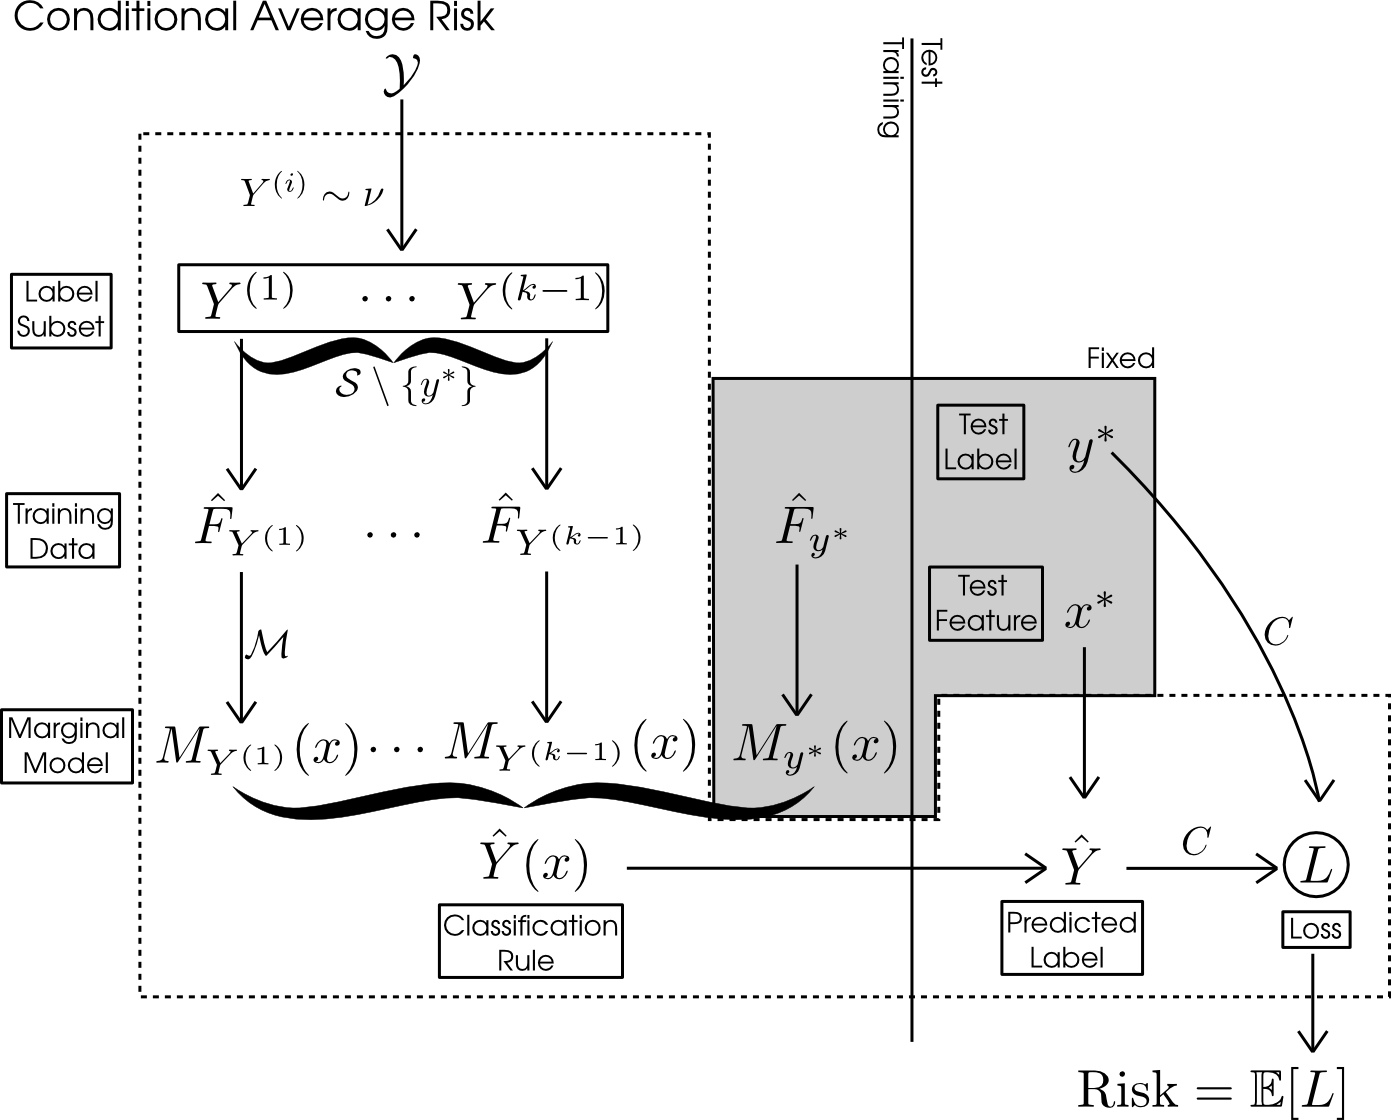
\includegraphics[scale = 0.3]{../extrapolation_figures/conditional_risk.png}
\caption{Conditional average risk}\label{fig:conditional_risk}
\end{figure}

%However, we will further decompose $R_k$ into $k$-dependent and $k$-independent components.
%Having defined the conditional average risk, we will now further
%decompose it to expose its dependence on $k$.
Now, in order to analyze the $k$-class behavior of the conditional
average risk, we begin by considering the \emph{two-class} situation.

In the two-class situation, we have a true label $y^*$ and one
incorrect label, $Y$.  Define the \emph{U-function}
$U_{x^*}(y^*, \hat{F}_{y^*})$ as the \emph{probability of correct
classification} in the two-class case.
The classification is correct if the margin
$M_{y^*}(x^*)$ is greater than the margin $M_Y(x^*)$, and incorrect
otherwise.  
Since we are fixing $x^*$ and $(y^*, \hat{F}_{y^*})$, the
probability of correct classification is obtained by taking an expectation:
\begin{align}\label{eq:U_function}
U_{x^*}(y^*, \hat{F}_{y^*}) &= \Pr[M_{y^*}(x^*) > \mathcal{M}(\hat{F}_Y)(x^*)]
\\&= \int_{\mathcal{Y}} 
I\{
M_{y^*}(x^*) > \mathcal{M}(\hat{F}_{y})(x)
\}
d\Pi_{y, r}(\hat{F}_y)
d\pi(y).
\end{align}
See also figure \ref{fig:U_function} for an graphical illustration of
the definition.

\begin{figure}[h]
\centering
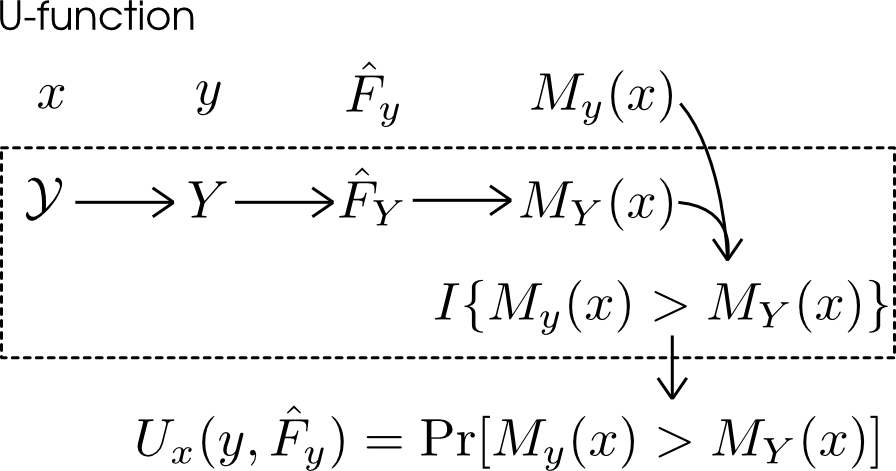
\includegraphics[scale = 0.4]{../extrapolation_figures/U_function.png}
\caption{U-functions}\label{fig:U_function}
\end{figure}

An important property of the U-function, and the basis for its name,
is that the random variable $U_x(Y, \hat{F}_Y)$ for $Y \sim \pi$ and
$\hat{F}_Y \sim \Pi_{Y, r}$ is uniformly distributed for all
$x \in \mathcal{X}$.  This is proved in Lemma \ref{lemma:U_function}
in the appendix.

Now, we will see how the U-function allows us to understand the
$k$-class case.  Suppose we have true label $y^*$ and incorrect labels
$Y^{(1)},\hdots, Y^{(k-1)}$.  Note that the U-function
$U_{x^*}(y, \hat{F}_y)$ is monotonic in $M_y(x^*)$.  Therefore,
\[
\hat{Y} = \argmax_{y \in \mathcal{S}} M_y(x^*) = \argmax_{y \in \mathcal{S}} U_{x^*}(y, \hat{F}_y).
\]
Therefore, we have a correct classification if and only if the U-function value for the correct label
is greater than the maximum U-function values for the incorrect labels:
\[
\Pr[\hat{Y} = y^*] = \Pr[U_{x^*}(y^*, \hat{F}_{y^*}) > \max_{i=1}^{k-1} U_{x^*}(Y^{(i)}, \hat{F}_{Y^{(i)}})] =  \Pr[u^* > U_{max}].
\]
where $u^* = U_{x^*}(y^*, \hat{F}_{y^*})$ and $U_{max, k-1}
= \max_{i=1}^{k-1} U_{x^*}(Y^{(i)}, \hat{F}_{Y^{(i)}})$.  But now,
observe that we know the distribution of $U_{max, k-1}$!  Since
$U_{x^*}(Y^{(i)}, \hat{F}_{Y^{(i)}})$ are i.i.d. uniform, we know that
\begin{equation}\label{eq:umax_beta}
U_{max, k-1} \sim \text{Beta}(k-1, 1). 
\end{equation}
We now have the insights needed to analyze the simplest special case: zero-one loss.
\newline

\noindent \emph{Special case: 0-1 loss}.
For zero-one loss, which is $C(y, y') = I\{y = y'\}$, we have $L=1$ if
and only if $U_{max} > u^*$ and $L=0$ otherwise.  Therefore, the
conditional average risk is
\[
\text{CondRisk}_k((y^*, \hat{F}_{y^*}), x^*) = \Pr[U_{max} > u^*] = \int_{u^*}^1 (k-1) u^{k-2} du.
\]
Now the average risk can be obtained by integrating over the distribution of $U^* = U_{x^*}(y^*, \hat{F}_{y^*})$.
We have
\begin{align*}
\text{AvRisk}_k &= \E[ \int_{U^*}^1 (k-1) u^{k-2} du] 
\\&= \E[\int_0^1 I\{u \geq U^*\} (k-1) u^{k-2} du ]
\\&= (k-1) \int_0^1 \Pr[U^* \leq u] u^{k-2} du.
\end{align*}
Or equivalently,
\[
\text{AvRisk}_{k, r, \nu}((y^*, \hat{F}_{y^*}), x^*) = (k-1) \int \bar{D}(u) u^{k-2} du.
\]
where $\bar{D}(u)$ denote the cumulative distribution function of $U^*$ on $[0,1]$:
\[
\bar{D}(u) = \Pr[U_{x^*}(y^*, \hat{F}_{y^*}) \leq u].
\]
We have expressed the average risk expressed as a weighted integral of
a certain function $\bar{D}(u)$ defined on $u \in [0,1]$.  We have
clearly isolated the part of the average risk which is independent of
$k$--the univariate function $\bar{D}(u)$, and the part which is
dependent on $k$--which is the density of $U_{max}$.

In section \ref{sec:estimation}, we will develop estimators of
$\bar{D}(u)$ in order to estimate the $k$-class average risk.
But now let us return to the general case.
\newline

\noindent \emph{General loss functions.}
The case for general cost functions is somewhat more complicated,
since knowledge of $U_{max}$ is not sufficient to determine $L$.  In
short, this is because $U_{max}$ by itself is insufficient to
determine $\hat{Y}$, and therefore $L=C(\hat{Y}, y^*)$.  However, we
can resolve this issue by noting that for the purposes of computing
the expected loss, it suffices to have the \emph{conditional
distribution} of $\hat{Y}$ given $U_{max}$.  Even though $U_{max}$
does not deterministically map onto a unique $\hat{Y}$, it determines
a conditional distribution of $\hat{Y}$ which allows us to compute
$\E[L|U_{max}, x^*, y^*, \hat{F}_{y^*}]$.

Now, a key fact is that the conditional distribution of $\hat{Y}$
given $U_{max}$ \emph{does not depend} on $k$.  To see this fact,
suppose without loss of generality that $\hat{Y} = Y^{(k-1)}.$ Then
the joint density of $Y^{(1)},\hdots, Y^{(k-1)}$ given $U_{max} =
u$ can be written
\[
p(y^{(1)},\hdots, y^{(k-1)}) \propto 
\pi(y^{(k-1)})\frac{d}{dt}\Pr[U_{x^*}(y^{(k-1)}, \hat{F}_{y^{(k-1)}}) \leq t]|_{t=u}
\prod_{i=1}^{k-2}\pi(y^{(i)})\Pr[U_{x^*}(y^{(k-1)}, \hat{F}_{y^{(k-1)}}) < u].
\}
\]
up to a normalizing constant.  Note that the term
$\frac{d}{dt}\Pr[U_{x^*}(y^{(k-1)}, \hat{F}_{y^{(k-1)}}) \leq t]$ is the
density of the random variable
$U_{x^*}(Y^{(k-1)}, \hat{F}_{Y^{(k-1)}})$. From the density, we can see
that $Y^{(1)},\hdots, Y^{(k-1)}$ are conditionally independent given
$U_{max} = u$, hence the marginal density of $\hat{Y}=Y^{(k-1)}$ can
be written
\[
p(\hat{y}) \propto \pi(\hat{y})\frac{d}{dt}\Pr[U_{x^*}(y^{(k-1)}, \hat{F}_{y^{(k-1)}}) \leq t]|_{t=u}.
\]

The only property of the conditional distribution of $\hat{Y}|U_{max} = u$ that is needed is
the expectation of $L = C(\hat{Y}, y^*)$.  Therefore, define the \emph{conditional expected loss} $D((y^*, \hat{F}_{y^*}), x^*, u)$ by
\begin{equation}\label{eq:Kfunc}
D((y^*, \hat{F}_{y^*}), x^*, u) = \begin{cases} 0 \text{ if } u < u^*\\
\E[C(\hat{Y}, y^*)|U_{max} = u, x^*, y^*, \hat{F}_{y^*}] \text{ otherwise.}
\end{cases}
\end{equation}
We have the two cases $u < u^*$ and $u > u^*$ since when $U_{max} <
u^*$, the correct label is chosen and the loss is zero.  Otherwise, an
incorrect label is chosen, and the expected loss must be calculated
using the conditional distribution of $\hat{Y}$.

Again, since the conditional distribution of $\hat{Y}|U_{max}, x^*,
(y^*, \hat{F}_{y^*})$ is independent of $k$, the conditional cost
function is also independent of $k$.

With the conditional cost function and the distribution of $U_{max}$ both in hand, we can compute the average conditional risk
\[
\text{CondRisk}_k((y^*, \hat{F}_{y^*}), x^*) = (k-1) \int D((y^*,\hat{F}_{y^*}), x^*, u) u^{k-2} du.
\]
Now the average risk can be obtained by integrating over $(Y^*, \hat{F}_{Y^*}),$ and $X^*$.
\[
\text{AvRisk}_{k, r} = (k-1) \int \bar{D}(u) u^{k-2} du.
\]
where
\begin{equation}\label{eq:Kbar}
\bar{D}(u) = \int D((y^*,\hat{F}_{y^*}), x^*, u) \pi(y^*)dy dF_{y^*}(x^*) d\Pi_{y^*, r}(\hat{F}_{y^*}).
\end{equation}


This is the key result behind our estimation method, which was stated in theorem \ref{theorem:avrisk_identity}. 
The proof is given in the appendix.

Having this theoretical result allows us to understand how the
expected $k$-class risk scales with $k$ in problems where all the
relevant densities are known.  However, applying this result in
practice to estimate $\text{Average Risk}_k$ requires some means of
estimating the unknown function $\bar{D}$--which we discuss in the
following.

\section{Estimation}

Now we address the problem of estimating $\text{AvRisk}_{k_2,
r_{train}}$ from data.  As we have seen from
Theorem \ref{theorem:avrisk_identity}, the $k$-class average risk of
a marginal classifier $\mathcal{M}$ is a functional of a object called
$\bar{D}(u),$ which depends marginal model $\mathcal{M}$ of the
classifier, the joint distribution of labels $Y$ and features $X$ when
$Y$ is drawn from the sampling density $\nu$.

Therefore, the strategy we take is to attempt to estimate $\bar{D}$
for then given classification model, and then plug in our estimate of
$\bar{D}$ into the integral \eqref{eq:avrisk_identity} to obtain an
estimate of $\text{AvRisk}_{k_2, r_{train}}$.

Having decided to estimate $\bar{D}$, there is then the question of
what kind of model we should assume for $\bar{D}$.  While a
nonparametric approach may be ideal, for the case of general loss
functions we will adopt a parametric model: that is the subject of
this section.
%On the other
%hand, for the special case of zero-one loss
%(Section \ref{sec:sp_case}), we take a nonparametric approach.

Let us assume the linear model
\begin{equation}\label{eq:linearKu}
\bar{D}(u) = \sum_{\ell = 1}^m \beta_\ell h_\ell(u),
\end{equation}
where $h_\ell(u)$ are known basis functions, and $\beta$ are the model
parameters to be estimated. We can obtain \emph{unbiased} estimation
of $\text{AvRisk}_{k_2, r_{train}}$
%.  The first approach estimates the
%coefficients $\beta$ 
via the unbiased estimates of $k$-class average risk obtained from \eqref{eq:avtestrisk}.
%The second approach estimates $\beta$ by
%estimating $\bar{D}(u)$ directly.  However, the second approach
%requires the use of the \emph{regression adjustment} method taken from
%measurement error models, and therefore can only yield unbiased
%estimates for \emph{polynomial} basis functions $h_\ell(u)$.

If we plug in the assumed linear model \eqref{eq:linearKu} into the
identity \eqref{eq:avrisk_identity}, then we get
\begin{align}
\text{AvRisk}_{k, r_{train}} &= (k-2)\int \bar{D}(u) u^{k-2} du
\\&= (k-2)\int_0^1 \sum_{\ell = 1}^m \beta_\ell h_\ell(u) u^{k-2} du
\\&= \sum_{\ell = 1}^m \beta_\ell H_{\ell,k} \label{eq:avrisk_linear}
\end{align}
where
\begin{equation}
H_{\ell,k} = (k-2) \int_0^1 h_\ell(u) u^{k-2} du.
\end{equation}
The constants $H_{\ell, k}$ are moments of the basis function
$h_\ell$: hence we call this method the \emph{moment method.}  Note
that $H_{\ell, k}$ can be precomputed numerically for any $k \geq 2$.


Now, since the $\text{AvTestRisk}_k$ are unbiased estimates of
$\text{AvRisk}_{k, r_{train}}$, this implies that the regression
estimate
\[
\hat{\beta} = \argmin_\beta \sum_{k=2}^{k_1} w_k \left(\text{AvTestRisk}_k - \sum_{\ell=1}^m \beta_\ell H_{\ell, k}\right)^2
\]
is unbiased for $\beta$, under any choice of positive weights $w_k$.
The estimate of $\text{AvRisk}_{k_2,r_{train}}$ is similarly obtained
from \eqref{eq:avrisk_linear}, via
\begin{equation}\label{eq:avrisk_hat}
\widehat{\text{AvRisk}_{k_2,r_{train}}} = \sum_{\ell=1}^m \hat{\beta}_\ell H_{\ell, k_2}.
\end{equation}

\subsection{Large-Sample Theory}

How good are the estimated average risks \eqref{eq:avrisk_hat}?  Let
us investigate the accuracy of the estimates in the limit where
$k_1 \to \infty$, first in the case where the
model \eqref{eq:linearKu} is correctly specified, and then considering
possible model misspecification.

If we fix the number of classes $k_2$ which defines the estimation
target, then we need not use the estimator \eqref{eq:avrisk_hat},
since once $k_1 > k_2$, we can use the $\text{AvTestRisk}_{k_2}$ as an
estimator instead, which can easily be shown to a have a convergence
rate of $O(1/\sqrt{k_1})$ to the true average risk.  Therefore, if we
want to quantify the performance of the regression-based
estimator \eqref{eq:avrisk_hat}, it does not make sense to look at
asymptotic settings where $k_2$ is fixed.  One approach is to specify
a setting where $k_2$ changes as a function of $k_1$.  However, the
approach we will take is to look at the minimax error: that is, to
look at the maximum discrepancy between the estimate and the true
average risk over all $k_2$ simultaneously.  The performance criterion
is the minimax error, defined
\begin{equation}\label{eq:minimax_error}
\text{MinimaxError} = \sup_{k_2 > 2} |\widehat{\text{AvRisk}_{k_2,r_{train}}} - \text{AvRisk}_{k_2,r_{train}}|.
\end{equation}

\noindent\emph{Well-specified case.}

Let us first assume that the parametric model \eqref{eq:linearKu} is correct. Then
\[
\text{AvRisk}_{k_2,r_{train}} = \sum_{\ell=1}^m \beta_\ell H_{\ell, k_2} = \langle \vec{H}_{k_2}, \beta \rangle
\]
where $\vec{H}_{k_2} = (H_{\ell, k_2})_{\ell=1}^m$.
Then, we get
\[
\text{MinimaxError} = \sup_{k_2 > 2} |\langle \vec{H}_{k_2}, \beta - \hat{\beta}\rangle|.
\]
If we assume that all the basis functions $h_\ell(u)$ are bounded by a
common constant $M$, then it follows that $H_\ell, k$ are also bounded by the same constant $M$,
and we have
\[
\text{MinimaxError} \leq M ||\beta - \hat{\beta}||_1 \leq M \sqrt{m}||\beta - \hat{\beta}||_2
\]

Therefore, any convergence rate we can establish for $\hat{\beta}$ is
inherited by the minimax error.  Meanwhile, we can show that choosing
$k_0$ sufficiently large that $(\vec{H}_2,\hdots,\vec{H}_{k_0})$ is
full-rank, and setting weights $w_k = I\{k \leq k_0\}$, then the
resulting $\hat{\beta}$ converges to the true $\beta$ at the usual
$O(1/\sqrt{n})$ rate.  We state the result in the following theorem.

\begin{theorem}
Consider a sequence of problems where the model $\mathcal{M}$,
$r_{train}$, $r_{test}$, joint distribution
$\{F_y\}_{y \in \mathcal{Y}}$, and class sampling distribution $\eta$
are fixed as $k_1 \to \infty$.  Further assume that the function
$\bar{D}(u)$ defined by $\{F_y\}_{y \in \mathcal{Y}}$, $\eta$, and
$\mathcal{M}$ satisfies
\[
\bar{D}(u) = \sum_{\ell = 1}^m \beta_\ell h_\ell(u)
\]
for some basis functions $h_\ell(u)$.
%and that those basis functions satisfy
%\[
%\max_{\ell=1}^m ||h_\ell(u)||_\infty < M
%\]
%for some constant $M < \infty$.
Let $k_0$ be an integer sufficiently large so that
\[
\text{Rank}(\vec{H}_2,\hdots,\vec{H}_{k_0}) = m.
\]
Then, defining
\[
\hat{\beta} = \argmin_\beta \sum_{k=2}^{k_0} \left(\text{AvTestRisk}_k - \sum_{\ell=1}^m \beta_\ell H_{\ell, k}\right)^2
\]
there exists some constant $C < \infty$ such that
\[
\lim_{k_1 \to \infty} \sqrt{k_1}||\hat{\beta}-\beta||_2 = C.
\]
\end{theorem}

\textbf{Proof.}
Note that the statistics $\text{AvTestRisk}_k$ are U-statistics of the
$k_1$ pairs of test and training samples.  Therefore, by Hoeffding
1948, it follows that
$(\text{AvTestRisk}_2,\hdots, \text{AvTestRisk}_{k_0})$ is
asymptotically normal with covariance satisfying
\[
\lim_{k_1 \to \infty} k_1 \Cov(\text{AvTestRisk}_2,\hdots, \text{AvTestRisk}_{k_0}) = \Sigma,
\]
for some positive semidefinite matrix $\Sigma$.  Defining $\bH$ to be
the matrix with rows $\vec{H}_2,\hdots,\vec{H}_{k_0}$, this then
implies that
\[
\lim_{k_1 \to \infty} k_1 \Cov(\hat{\beta}) = (\bH^T \bH)^{-1} \bH^T \Sigma \bH (\bH^T \bH)^{-1}.
\]
It follows that defining
\[
C = \sqrt{\text{tr} (\bH^T \bH)^{-1} \bH^T \Sigma \bH (\bH^T \bH)^{-1}}
\]
we have
\[
\lim_{k_1 \to \infty} \sqrt{k_1}||\hat{\beta}-\beta||_2 = C.
\]
$\Box$.

\noindent\emph{Misspecified case.}

Now consider the more realistic setting where the
model \eqref{eq:linearKu} is misspecified.  We quantify the degree of
misspecification by the $\ell_\infty$ error on [0,1].  Define
\[
\delta = \inf_{\beta} \|\bar{D}(u) - \sum_{\ell = 1}^m \beta_\ell h_\ell(u)\|_\infty,
\]
and let $\tilde{\beta}$ be the coefficients $\beta$ which attain the infimum,
with $\tilde{D}(u) = \sum_{\ell = 1}^m \tilde{\beta}_\ell h_\ell(u)$.
To deal with this case, refer to the theory in section \ref{sec:misspecifiedOLS}.
For each $u = [0,1]$, find a matrix $A(u)$ such that (i) the first column equals
\[
A_1(u) = (h_1(u),\hdots, h_m(u))
\]
and that (ii) the rest of the columns are orthogonal to the first,
and (iii) $A(u)$ is full-rank.
Then define $Z(u) = X A(u)$,
and consider the column vector
\[
Z_{1|-1}(u) = (I - P_{Z_{-1}}) Z_1(u).
\]
It can be shown that $Z_{1|-1}(u)$ is well-defined, regardless of how
$A(u)$ is chosen.  Then, by the theory in section \ref{sec:misspecifiedOLS},
the extra bias due to approximation error for predicting $\hat{D}(u)$
is given by
\[
\text{Bias}^2(u) = \frac{||Z_{1|-1}(u)||_1^2}{||Z_{1|-1}(u)||_2^4}.
\]
Define the maximum bias as
\[
\text{Bias}^2_{max} = \sup_{ u \in [0,1]} \text{Bias}^2(u).
\]
From the analysis of the well-specified case, we know that the
variance component of the prediction risk decreases at order $O(1/k)$.
Therefore, the misspecified minimax error is of order
\[
\text{MinimaxError} = O(1/\sqrt{k}) + \text{Bias}^2_{max}.
\]


\section{Examples}

